\providecommand{\main}{../../main}
\documentclass[../../main.tex]{subfiles}

\usepackage{tikz-feynman}

\begin{document}

\chapter{Introduction}
    
\label{sec:introduction}
    
    
The \acrfull{hllhc} will open an unprecedented window on the weak-scale nature of the universe, providing high-precision measurements of the standard model electroweak interaction, including properties of the Higgs Boson, as well as searches for new physics beyond the standard model. The new requirements in terms of rate and latency exceed the present capabilities of the front-end and back-end electronics forcing the entire replacement of the \acrshort{cms} main parts including the trigger system.
    
The \acrshort{hllhc}, will start operating after the third Long Shutdown (\acrshort{ls3}), and is designed to provide an increased instantaneous luminosity, at the price of extreme pileup of interactions. In \acrshort{ls3}, the \acrshort{cms} detector will also undergo a major upgrade to prepare for the so called Phase-2 of the \acrshort{lhc} physics program, starting in 2029.
    
Aim of the proposed thesis is to contribute to the development of a new Level-1 (L1) trigger for the \acrshort{cms} Experiment, in particular on the new \acrfull{gt} subsystem. The \acrshort{cms} trigger system is made of two trigger levels. The \acrfull{l1t} the first step of event reduction, based on physics selections, the second step to further reduce the stored events is done by the \acrfull{hlt}. The L1 hardware consists of custom programmable electronics working at local, regional and global scale. Within L1, the Global Trigger (\acrshort{gt}, top entity of the hierarchy) is responsible for selecting events to be processed by the following software trigger stage. \acrshort{hlt} on the other end employs of the shelves electronics within on site computing farm. 
    
The work presented on this thesis is focused on the GT, which its decision is presently based on calculations of physics parameters applied to candidate particles and global parameters. Such algorithms range from setting thresholds on transverse (p, E) on single objects to more complex calculations based on multiplicities and topological conditions.  
    
The new \acrshort{gt} shall consist of multiple processors, each receiving the full set of trigger objects, but calculating different set of algorithms, namely the \textit{trigger menu}. The use of advanced object identification algorithms, including machine learning and multivariate analysis techniques, will facilitate greater use of object classification variables in the \acrshort{gt}.
    
The LHC schedule is shown in Fig. \ref{fig:lhc-plan}, study and test are already taking place at CERN to verify new concepts and algorithms before the upgrade commissioning.
    
\begin{figure}[h]
    \centering
    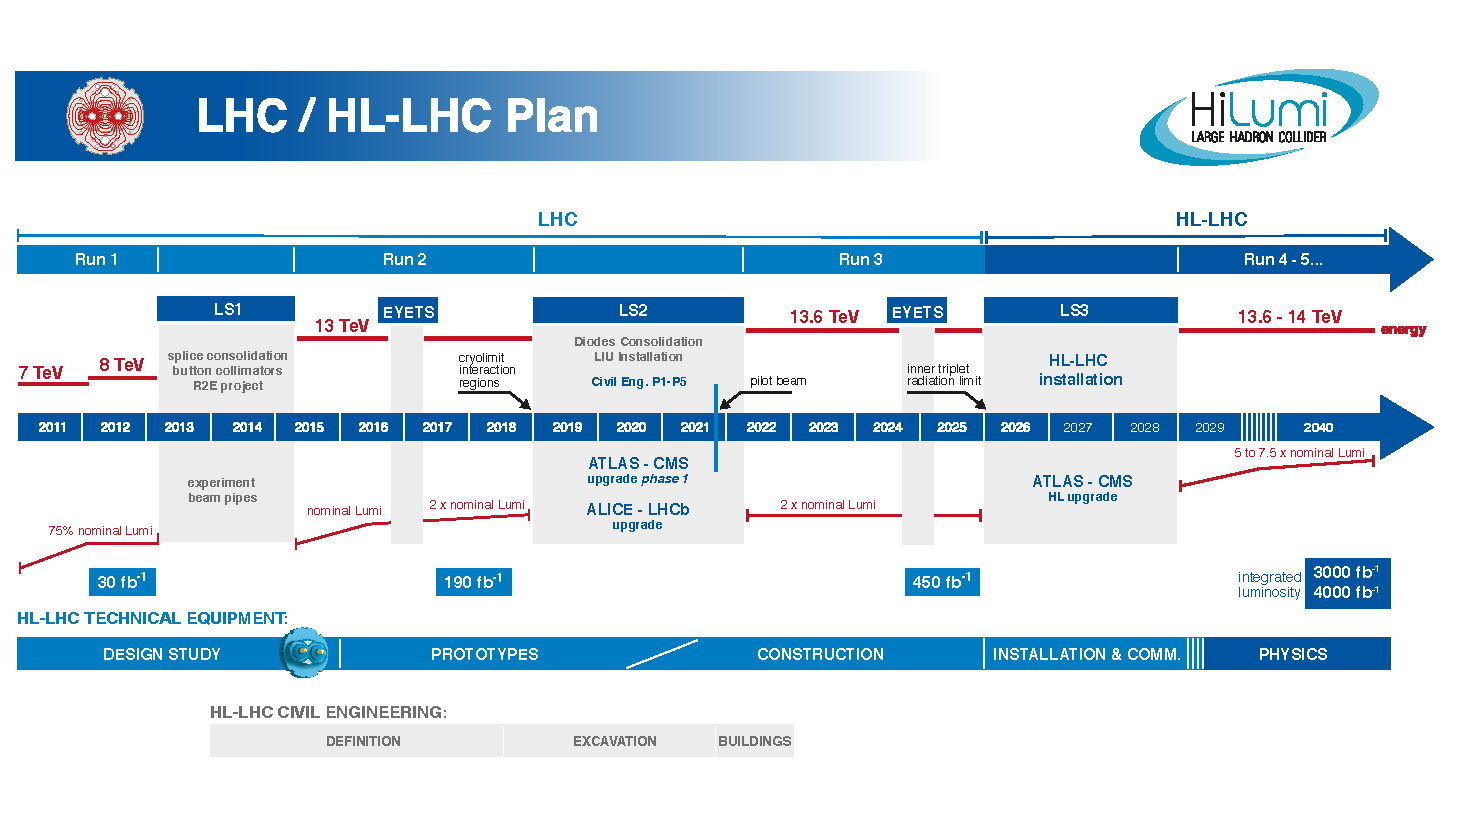
\includegraphics[width=0.97\textwidth]{sections/01/Images/HL-LHC_Janvier2022.pdf}
    \caption{LHC upgrade plan.}
    \label{fig:lhc-plan}
\end{figure}
    
The thesis work will be sub-divided in two main branches.
    
Firstly a new types of algorithms will be studied in the \acrshort{hllhc} setup, namely the neural networks based algorithm. To do so, \textit{hls4ml} tool will be employed to perform the translation from high level programming code (Python and Keras) to \acrfull{hls}. The \acrshort{hls} code will be  integrated in the GT firmware to produce a bit-file to be loaded on the target \acrfull{fpga} boards. The algorithms produced will be firstly simulated in software, then tested on standalone firmware and only if the results are satisfactory will be tested and implemented in the GT firmware.
    
Secondly the Final-OR (finor) board firmware is be developed, this board has the aim to monitor and eventually pre-scale the incoming $\sim$1000 different algorithms alongside this monitoring and conditioning msaks are applied, then they will be merged and up to 8 different trigger types are produced. These trigger types are chosen according to the physics program needed.  
    
The VHDL code currently implemented in the present Global Trigger board, developed by the Vienna \acrshort{cms} group, will be revisited and modified to match the updated features of the Phase-2 upgrade. Firstly the firmware must be revisited and optimized where possible, since in the Final-OR logic will be deployed in an upgraded version of the current used FPGA (Virtex-7 $\to$ Virtex-Ultrascale$+$) and with more that double the algorithms.  
    
    %Secondly, new feature will be added to meet the new requirements of the Phase-2 upgrade in therms of increased trigger rate, number of algorithms and input data throughput. 
    
    %Lastly the interface to the Timing and Control Distribution System (TCDS-2) must be developed and implemented in the finor board to distribute the trigger signals (multiple trigger Physics) to the detector readout electronics.
    



    

\end{document}